../cictikz/src/cictikz/data/tex/cictikz_preamble.tex

% Drain current against gate voltage, on a log current axis.
%
% Six decades of current over less than two volts of gate. The straight
% part below threshold is weak inversion, where the gate is moving a
% barrier and the current is exponential in gate voltage; above threshold
% the curve bends over as the channel becomes a resistance instead.
%
% A linear axis would show only the top decade, which is why this plot is
% always drawn on a log one, and why a transistor that looks firmly off on
% a linear plot is still passing nanoamps.
%
% Generated by py/tikzplot.py. Edit the script in ex/ that
% produced it and re-run that, not this file.

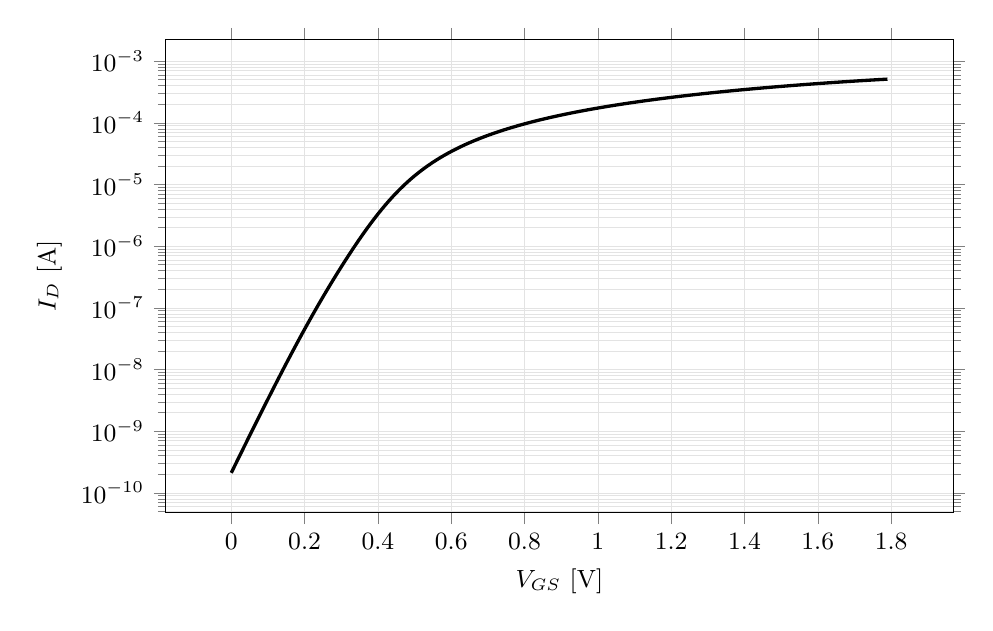
\begin{tikzpicture}[thick]

\begin{axis}[
  width=10.0cm,
  height=6.0cm,
  scale only axis,
  grid=both,
  grid style={gray!22, very thin},
  tick align=outside,
  tick label style={font=\small},
  label style={font=\small},
  title style={font=\small, yshift=-1mm},
  legend cell align=left,
  legend style={font=\small, draw=gray!50, fill=white, fill opacity=0.85, text opacity=1},
  ymode=log,
  xlabel={$V_{GS}$ [V]},
  ylabel={$I_D$ [A]}
]
\addplot[black, very thick, mark=none] coordinates {(0,2.1147e-10) (0.01,2.7934e-10) (0.02,3.6881e-10) (0.03,4.8669e-10) (0.04,6.4186e-10) (0.05,8.4592e-10) (0.06,1.114e-09) (0.07,1.4658e-09) (0.08,1.9267e-09) (0.09,2.5298e-09) (0.1,3.3177e-09) (0.11,4.3449e-09) (0.12,5.6816e-09) (0.13,7.4171e-09) (0.14,9.6647e-09) (0.15,1.2568e-08) (0.16,1.6307e-08) (0.17,2.1109e-08) (0.18,2.7256e-08) (0.19,3.5096e-08) (0.2,4.5064e-08) (0.21,5.769e-08) (0.22,7.3627e-08) (0.23,9.367e-08) (0.24,1.1879e-07) (0.25,1.5016e-07) (0.26,1.8921e-07) (0.27,2.3765e-07) (0.28,2.9755e-07) (0.29,3.7137e-07) (0.3,4.6205e-07) (0.31,5.7302e-07) (0.32,7.083e-07) (0.33,8.7248e-07) (0.34,1.0707e-06) (0.35,1.3085e-06) (0.36,1.5923e-06) (0.37,1.9286e-06) (0.38,2.3242e-06) (0.39,2.7862e-06) (0.4,3.3215e-06) (0.41,3.9366e-06) (0.42,4.6377e-06) (0.43,5.4304e-06) (0.44,6.3194e-06) (0.45,7.3085e-06) (0.46,8.4007e-06) (0.47,9.5981e-06) (0.48,1.0902e-05) (0.49,1.2312e-05) (0.5,1.3828e-05) (0.51,1.5449e-05) (0.52,1.7173e-05) (0.53,1.8998e-05) (0.54,2.0922e-05) (0.55,2.2941e-05) (0.56,2.5053e-05) (0.57,2.7254e-05) (0.58,2.9542e-05) (0.59,3.1913e-05) (0.6,3.4364e-05) (0.61,3.6893e-05) (0.62,3.9496e-05) (0.63,4.217e-05) (0.64,4.4914e-05) (0.65,4.7723e-05) (0.66,5.0596e-05) (0.67,5.3531e-05) (0.68,5.6524e-05) (0.69,5.9575e-05) (0.7,6.268e-05) (0.71,6.5838e-05) (0.72,6.9048e-05) (0.73,7.2306e-05) (0.74,7.5613e-05) (0.75,7.8965e-05) (0.76,8.2362e-05) (0.77,8.5801e-05) (0.78,8.9282e-05) (0.79,9.2804e-05) (0.8,9.6363e-05) (0.81,9.9961e-05) (0.82,0.00010359) (0.83,0.00010726) (0.84,0.00011097) (0.85,0.0001147) (0.86,0.00011847) (0.87,0.00012226) (0.88,0.00012609) (0.89,0.00012995) (0.9,0.00013383) (0.91,0.00013774) (0.92,0.00014167) (0.93,0.00014563) (0.94,0.00014962) (0.95,0.00015362) (0.96,0.00015765) (0.97,0.0001617) (0.98,0.00016577) (0.99,0.00016986) (1,0.00017397) (1.01,0.0001781) (1.02,0.00018224) (1.03,0.0001864) (1.04,0.00019058) (1.05,0.00019477) (1.06,0.00019898) (1.07,0.0002032) (1.08,0.00020744) (1.09,0.00021168) (1.1,0.00021594) (1.11,0.00022022) (1.12,0.0002245) (1.13,0.00022879) (1.14,0.00023309) (1.15,0.00023741) (1.16,0.00024173) (1.17,0.00024606) (1.18,0.0002504) (1.19,0.00025474) (1.2,0.00025909) (1.21,0.00026345) (1.22,0.00026781) (1.23,0.00027218) (1.24,0.00027656) (1.25,0.00028093) (1.26,0.00028532) (1.27,0.0002897) (1.28,0.00029409) (1.29,0.00029848) (1.3,0.00030288) (1.31,0.00030727) (1.32,0.00031167) (1.33,0.00031607) (1.34,0.00032047) (1.35,0.00032487) (1.36,0.00032926) (1.37,0.00033366) (1.38,0.00033806) (1.39,0.00034246) (1.4,0.00034685) (1.41,0.00035124) (1.42,0.00035563) (1.43,0.00036002) (1.44,0.0003644) (1.45,0.00036878) (1.46,0.00037316) (1.47,0.00037753) (1.48,0.00038189) (1.49,0.00038625) (1.5,0.00039061) (1.51,0.00039495) (1.52,0.00039929) (1.53,0.00040363) (1.54,0.00040795) (1.55,0.00041227) (1.56,0.00041658) (1.57,0.00042088) (1.58,0.00042517) (1.59,0.00042946) (1.6,0.00043373) (1.61,0.00043798) (1.62,0.00044223) (1.63,0.00044647) (1.64,0.00045069) (1.65,0.0004549) (1.66,0.00045909) (1.67,0.00046327) (1.68,0.00046744) (1.69,0.00047159) (1.7,0.00047572) (1.71,0.00047983) (1.72,0.00048393) (1.73,0.00048801) (1.74,0.00049207) (1.75,0.00049611) (1.76,0.00050012) (1.77,0.00050412) (1.78,0.00050809) (1.79,0.00051204)};
\end{axis}

\end{tikzpicture}
\end{document}
